\section{Module Composition into Components and Architecture}
Module decomposition reduced \progname{}'s models into atomic units contained
in ``virtual'' modules that are not implemented (Levels 1 and 2 in
Table~\ref{TblMH}) but this is not necessarily how a user would visualize their
groupings. For example, the hierarchy does not group the Emotion Generation and
Emotion Intensity Function modules together despite their common dependencies
(Figure~\ref{FigUH}). A user might similarly view them as a single unit because
emotion intensity is only relevant if the associated emotion is present.
Therefore, \progname{}'s assignment of the 16 modules to eight components aims
to collect highly-related functionality into a comprehensive unit
(Figure~\ref{fig:components}) that can be exchanged for another with comparable
abilities while reducing inter-component connections
(Figure~\ref{fig:componentConnections}):
\begin{description}

    \item [\refstepcounter{cpnum} \mthecpnum \label{cpIntensity}:] Emotion
    Intensity collects the Emotion Intensity Type (\textbf{\mref{mIntensity}})
    and dependant Emotion State Type (\textbf{\mref{mStateType}}) modules
    because they represent \progname{}'s core emotion types. This also collects
    all \progname{}-specific models necessary for users to define custom
    emotion kinds (\rref{R_MixingEmotionsPES}, \rref{R_PartitionEmotions},
    \rref{R_MixingEmotionsCTE}). Since Emotion Intensity Type does not depend
    on other modules, this only reduces visible dependencies by one because the
    component hides Emotion State Type's dependency on Emotion Intensity Type.

    \item [\refstepcounter{cpnum} \mthecpnum \label{cpGenerate}:] Emotion
    Evaluation collects the Emotion Generation (\textbf{\mref{mGenerate}}) and
    Emotion Intensity Function (\textbf{\mref{mIntensityFun}}) modules due to
    the previously described interdependence of emotion generation and
    intensity calculations. Since these two modules require all the same
    inputs, grouping them as one unit also halves the visible dependencies on
    other modules.

    \item [\refstepcounter{cpnum} \mthecpnum \label{cpDecay}:] Emotion Decay
    collects the Emotion Intensity Decay (\textbf{\mref{mDecay}}) and Emotion
    State Decay (\textbf{\mref{mDecayState}}) because they capture the single
    ``decay emotion'' task. This hides Emotion State Decay's dependency on
    Emotion Intensity Decay while also halving the visible dependencies on other
    modules.

    \item [\refstepcounter{cpnum} \mthecpnum \label{cpEmotion}:] Emotion
    collects the Emotion Type (\textbf{\mref{mEmotionType}}) and Emotion
    Function (\textbf{\mref{mEmotionFun}}) modules because \progname{} intends
    the latter to be helper functions that make Emotion Type easier to use,
    effectively making Emotion Function wholly dependant on Emotion Type. This
    hides Emotion Function's dependency on Emotion Type while also halving the
    visible dependencies on other modules.

    \item [\refstepcounter{cpnum} \mthecpnum \label{cpPAD}:] PAD collects the
    PAD Type (\textbf{\mref{mPADType}}) and PAD Function
    (\textbf{\mref{mPADFun}}) modules because \progname{} only requires a PAD
    data type to contain an emotion state that the PAD Function module has
    transformed into a PAD point. Since PAD Type does not depend on other
    modules, this only reduces visible dependencies by one as the component
    hides PAD Function's dependency on PAD Type.

    \item [\refstepcounter{cpnum} \mthecpnum \label{cpTime}:] Time contains
    only the Time (\textbf{\mref{mTime}}) module. It is separated from the
    World State module (\textbf{\mref{mWorld}}) because there are significantly
    more dependencies on Time than World State, including ones that are
    otherwise independent of the world such as Emotion Decay
    (\textbf{\mref{mDecay}} and \textbf{\mref{mDecayState}}). Time does not
    depend on other modules, so there are no visible dependency reductions.

    \item [\refstepcounter{cpnum} \mthecpnum \label{cpWorld}:] World State
    contains only the World State (\textbf{\mref{mWorld}}) module due to the
    need for Time to be its own component. World State does not depend on other
    modules, so there are no visible dependency reductions.

    \item [\refstepcounter{cpnum} \mthecpnum \label{cpEntity}:] Entity contains
    the Goal (\textbf{\mref{mGoal}}), Plan (\textbf{\mref{mPlan}}), Social
    Attachment (\textbf{\mref{mSocial}}), and Attention
    (\textbf{\mref{mAttention}}) modules because of their common ``entity
    representation'' task. Unlike Time (\textbf{\mref{mTime}}) and World State
    (\textbf{\mref{mWorld}}), there is no need to separate them into different
    components due to a higher number of dependencies on one module and not the
    others. They are also all relied on by the Emotion Evaluation component
    (\textbf{C2}), so collecting the Entity modules together makes its use more
    convenient. There are no dependencies between Goal, Plan, Attention, or
    Social Attachment, so the component does not hide visible dependencies
    within itself. However, Goal and Plan's mutual dependency on World State
    (\textbf{\mref{mWorld}}) is visible as a single connection rather than two
    separate ones.

\end{description}

\vspace*{\fill}
\begin{figure}[!ht]
    \centering
    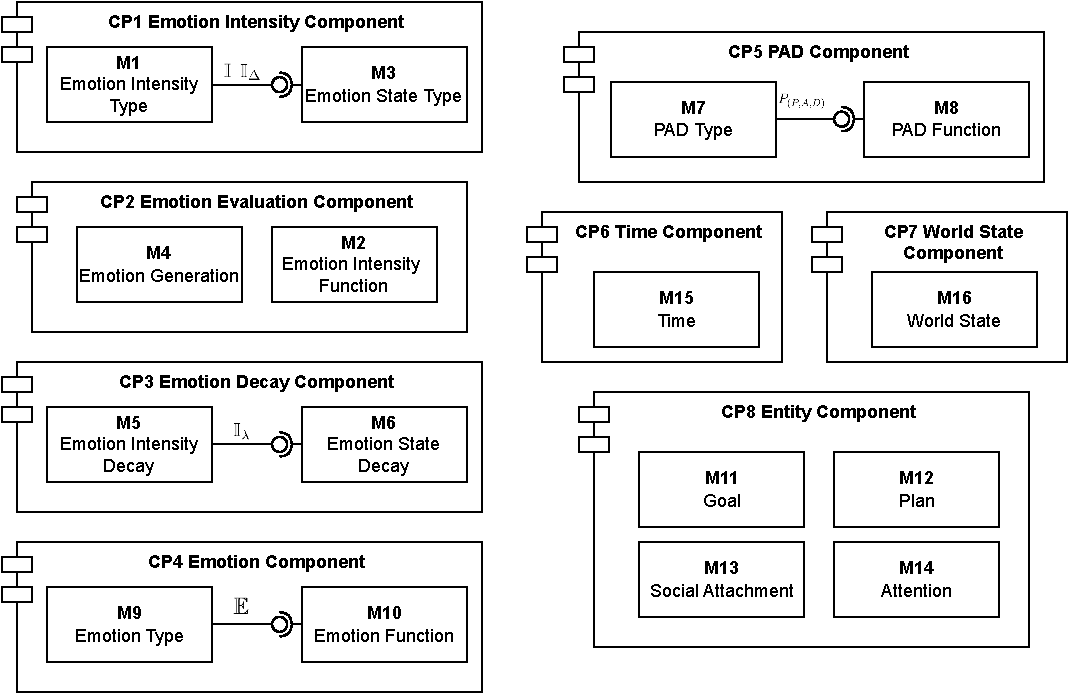
\includegraphics[width=\linewidth]{figures/emgineArch_internalComponents.pdf}
    \caption{Organization of Modules in Components (``Ball'' provides
    functionality that a ``Cup'' needs)}
    \label{fig:components}
\end{figure}
\vspace*{\fill}

\begin{figure}[!ht]
    \centering
    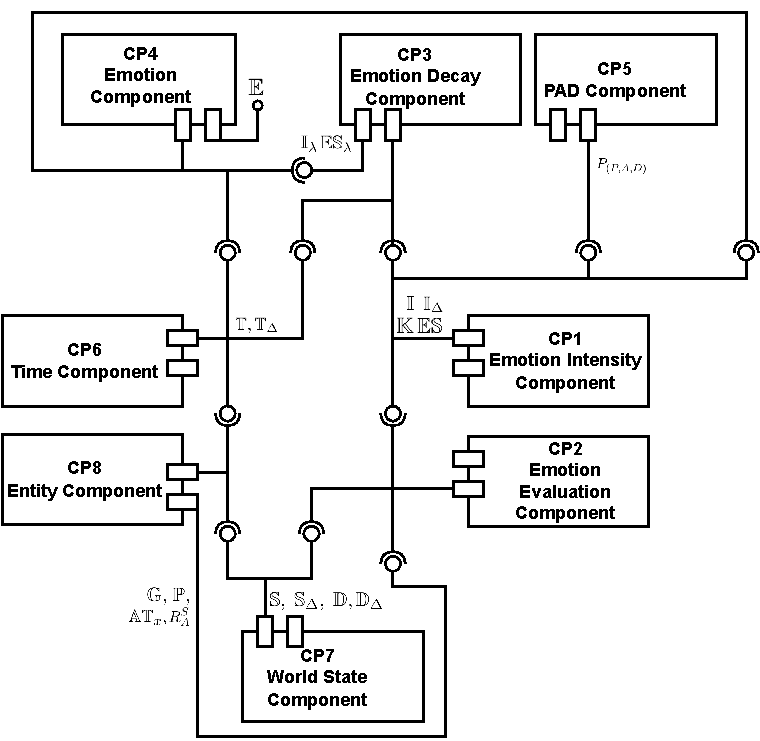
\includegraphics[width=0.7\linewidth]{figures/emgineArch_componentRelations.pdf}
    \caption{Relationships Between Modules (``Ball'' provides functionality
    that a ``Cup'' needs)}
    \label{fig:componentConnections}
\end{figure}